\scanpage{3}
\uline{Proposition}! Soient $S$ un schéma, $A$ un schéma abélien sur $S$,\\
$X$ un schéma sur $S$, \deleted{tel que \illegible{3} \unsure{géométriques}} \inserted{$\mathcal L$ un faisceau inversible sur} $A\times_S X$,\\
\deleted{Considérons l'homomorphisme}\\
trivial sur $e_A\times_S X$, et tel que \deleted{\unsure{pour que} \illegible{4}} pour tt\\
$x\in X$, le faisceau $\mathcal L_x$ sur $A_x=A_s\otimes_{k(s)}k(x)$ (où $s$ \unsure{pt|est} de $S$\\
sous $x$) soit alg. équivalent à zéro. Considérons l'application
\[
\varphi_{\mathcal L}:K^\bullet(A)\longrightarrow K^\bullet(X)
\]
définie par \deleted{l'application additive} le foncteur de catégories\\
triangulées $\Phi:D_{\unsure{\mathrm{parf}|\mathrm{prof}}}(A)\mathbin{-}D_{\unsure{\mathrm{parf}|\mathrm{prof}}}(X)$
\[
\Phi_{\mathcal L}(F)=\mathbf R\operatorname{pr}_{2*}\bigl(\mathbf L\operatorname{pr}_1^*(F)\otimes\mathcal L\bigr).
\]
Alors $\varphi_{\mathcal L}$ transforme produit de Pontryagin $*$ en\\
produit ordinaire. Plus précisément, on a un isomorphisme\\
de foncteurs de catégories triangulées
\[
\Phi_{\mathcal L}(F\overset{\mathbf L}{*}G)\simeq
\Phi_{\mathcal L}(F)\overset{\mathbf L}{\otimes}\Phi_{\mathcal L}(G)
\]
$(F,G\in\operatorname{Ob}D_{\unsure{\mathrm{parf}|\mathrm{prof}}}(A))$.

\figure{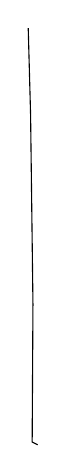
\begin{tikzpicture}[x=0.005cm,y=-0.005cm]
\draw (0,0)--(6,220)--(12,700)--(10,1050)--(24,1057);
\end{tikzpicture}}
\margin{peut se généraliser\\
au cas $A$ un\\
schéma en\\
groupes \inserted{plat}, $\mathcal L$\\
sur $A\times_S X$ satisfaisant\\
$(\pi_A\times\operatorname{id}_X)^*(\mathcal L)\simeq\operatorname{pr}_{13}^*(\mathcal L)\otimes\operatorname{pr}_{23}^*(\mathcal L)$\\
et $F$ et $G$ sur\\
$A$ à supports\\
propres sur $S$\\
et \deleted{\unsure{parf.}} \inserted{$F,G$}\\
$\in\operatorname{Ob}D_{\mathrm{qcoh}}(A)\ldots$\\
on peut enfin\\
généraliser en\\
\unsure{ou bien: accouplement}\\
\deleted{\unsure{un}} \unsure{accouplement}\\
de $C$-torseurs\\
$P\times Q\longrightarrow R$,\\
$C\times C\longrightarrow C$\\
et même pas\\
\unsure{besoin du groupe}\\
$C$, et partir de quelconques\\
faisceaux $\mathcal L,\mathcal L',\mathcal L''$\\
sur $R\times X,P\times X,Q\times X$,\\
\deleted{\unsure{tel}} \inserted{et $\pi:P\times Q\mathbin{-}R$,}\\
tels que \deleted{$\unsure{\mathbf R}$}\\
$(\pi\times\operatorname{id}_X)^*(\mathcal L)\simeq
\operatorname{pr}_{13}^*(\mathcal L')\overset{\mathbf L}{\otimes}
\operatorname{pr}_{23}^*(\mathcal L'')$}

Si le th. est démontré dans la situation donnée, il en\\
résulte qu'il est vrai dans tt situation \inserted{$(A,X',\mathcal L')$} qui s'en\\
déduit par image inverse à l'aide d'un $S$-morphisme\\
$g:X'\longrightarrow X$, car $\Phi_{\mathcal L'}\simeq\mathbf Lg^*(\Phi_{\mathcal L})$, et $\mathbf Lg^*$ commute à $\overset{\mathbf L}{\otimes}$.\\
\unsure{Soit} $B$ le schéma abélien dual de $A$, et $\mathcal L_0$ le\\
faisceau de Weil sur $A\times_S B$. Alors l'hypothèse sur $\mathcal L$\\
implique que $\mathcal L$ est $\simeq$ l'image inverse de $\mathcal L_0$ par un\\
$S$-morphisme $X\longrightarrow B$. Donc on est ramené au cas\\
où $X=B$, $\mathcal L=\mathcal L_0$. \deleted{\unsure{On}} On a des isom. fonctoriels
\[
(*)\qquad F\overset{\mathbf L}{\unsure{*|\otimes}}G=
\mathbf R\pi_{\unsure{*|\alpha}}(F\overset{\mathbf L}{\otimes}_S G)\qquad\text{et}
\]
\mspage{2}
